\chapter{Metodología y análisis de requisitos}
\label{ch:metodologia}

Este capítulo establece el marco metodológico del proyecto y formaliza los actores del sistema, los requisitos funcionales y no funcionales, los casos de uso y el diseño de la base de datos.

% ============================================================
\section{Metodología de desarrollo}
\label{sec:metodologia}

El \textit{modelo en cascada}\footnote{\textbf{Modelo en cascada}: Modelo de desarrollo secuencial en el que cada fase (análisis, diseño, desarrollo, pruebas y despliegue) debe cerrarse completamente antes de iniciar la siguiente. Su principal limitación es que asume que los requisitos pueden especificarse en su totalidad antes de escribir una sola línea de código.} fue descartado desde el inicio por una razón estructural importantísima: en un sistema con múltiples capas interdependientes (autenticación, geolocalización, pagos y aplicación nativa) la suposición de que todos los requisitos pueden conocerse antes de implementar es falsa. Especificar completamente el sistema antes de construirlo habría sido imposible en Parky, y tres episodios durante el desarrollo lo demuestran.

En primer lugar, el módulo \textit{SmartAccess} no figuraba en el análisis inicial y emergió en el sprint~4 porque al construir el flujo de reservas quedó claro que «el arrendatario llega al garaje y no puede entrar» era exactamente la fricción central que la plataforma pretendía eliminar. En segundo lugar, el \textit{trigger} de solapamiento de reservas se añadió en el sprint~8, no al principio ya que solo al implementar el flujo completo se hizo evidente que dos usuarios podían reservar la misma plaza simultáneamente. En tercer lugar, la auditoría de seguridad del sprint~7 detectó que el diseño de borrado de reservas destruía el historial financiero de los arrendadores, algo que solo resulta visible cuando el sistema maneja datos reales. En cascada, cualquiera de estos tres hallazgos habría obligado a reabrir la fase de requisitos y rediseñar desde arriba, con un coste de retroceso enorme.

Por ello se adoptó \textbf{Scrum}~\cite{scrum2020}\footnote{\textbf{Scrum}: Marco de trabajo ágil definido por Schwaber y Sutherland~\cite{scrum2020} que organiza el desarrollo en iteraciones de duración fija llamadas \textit{sprints}, al término de cada una de las cuales se entrega un incremento funcional del producto.} con \textit{sprints}\footnote{\textbf{Sprints}: Iteración de duración fija (dos semanas en Parky) al final de la cual se revisa el trabajo entregado, se ajusta el \textit{backlog} y se reprioriza el siguiente ciclo.} de dos semanas, cada uno centrado en un módulo de alto nivel. Scrum acepta que los requisitos evolucionan y lo convierte en una ventaja en lugar de un problema de modo que los errores que se detectan al final de cada ciclo, se corrigen en el siguiente sin afectar lo ya construido. Al tratarse de un proyecto unipersonal, los tres roles canónicos del marco (\textit{Product Owner}, \textit{Scrum Master} y equipo de desarrollo) convergieron en una única persona, y la retrospectiva de cada ciclo fue el mecanismo principal para detectar \textit{deuda técnica}\footnote{\textbf{Deuda técnica}: Coste futuro de corrección acumulado al tomar decisiones de implementación rápidas en lugar de óptimas. En un proyecto unipersonal, la retrospectiva de sprint es el único mecanismo formal para identificarla antes de que se propague.} antes de que se acumulara.

La Tabla~\ref{tab:sprints} recoge los nueve sprints en los que se desarrolló el prototipo, con sus respectivos módulos principales y entregables.

\begin{table}[h]
  \centering
  \caption{Sprints de desarrollo de Parky (enero--mayo de 2026).}
  \label{tab:sprints}
  \begin{tabularx}{\textwidth}{clXX}
    \toprule
    \textbf{Sprint} & \textbf{Período}    & \textbf{Módulo principal}
                    & \textbf{Entregable}                                                             \\
    \midrule
    \rowcolor{gray!5}
    1               & 6--19 ene           & Infraestructura base          & Scaffolding React/Vite,
    autenticación Supabase, rutas protegidas y modo oscuro.                                           \\
    2               & 20 ene--2 feb       & Modelo de datos y perfil      & Esquema de base de datos,
    RLS básico, edición de perfil e imágenes en Storage.                                              \\
    \rowcolor{gray!5}
    3               & 3--16 feb           & Plazas y mapa                 & Integración Leaflet,
    CRUD de garajes y plazas, React Query como capa de caché.                                         \\
    4               & 17 feb--2 mar       & Reservas, SmartAccess y pagos & Motor de precios, módulo
    SmartAccess con log de accesos y arquitectura de pagos.                                           \\
    \rowcolor{gray!5}
    5               & 3--16 mar           & Despliegue multiplataforma    & Vercel, compilación
    Android con Capacitor y APK nativo.                                                               \\
    6               & 17 mar--26 abr      & Memoria del TFG               & Redacción de los
    capítulos 1 a 4; commits de código suspendidos.                                                   \\
    \rowcolor{gray!5}
    7               & 27 abr--10 may      & Seguridad y calidad           & Auditoría de RLS,
    borrado lógico en \texttt{bookings} y HSTS/CSP en Vercel.                                         \\
    8               & 10--14 may          & Disponibilidad y reserva      & Horarios recurrentes,
    trigger de solapamiento y buffer de 15 minutos.                                                   \\
    \rowcolor{gray!5}
    9               & 15--19 may          & Pulido UX                     & \textit{Code splitting}
    (reducción del 95\,\% del \textit{bundle}), navegación inferior y
    \textit{touch targets} móvil.                                                                     \\
    \bottomrule
  \end{tabularx}
\end{table}

% ============================================================
\section{Actores del sistema}
\label{sec:actores}

En cuanto a los actores del sistema, Parky define cuatro roles principales definidos con claridad en la tabla~\ref{tab:actores-principales}. La separación entre arrendador y arrendatario no es solo conceptual sino también funcional, porque cada rol queda restringido a un subconjunto de datos distinto impuesto por las políticas RLS de la base de datos.

\begin{table}[H]
  \centering
  \caption{Actores del sistema Parky.}
  \label{tab:actores-principales}
  \begin{tabularx}{\textwidth}{lX}
    \toprule
    \textbf{Actor} & \textbf{Responsabilidades y alcance}                                                                                                                                             \\
    \midrule
    \rowcolor{gray!5}
    Arrendador     & Propietario de garajes. Publica plazas con precio, fotos y geolocalización. Acepta o rechaza reservas entrantes. Recibe pagos a través de Stripe Connect.                        \\
    \\
    Arrendatario   & Conductor que alquila plazas. Busca en el mapa, reserva, paga con Stripe y valora la plaza al finalizar.                                                                         \\
    \\
    \rowcolor{gray!5}
    Administrador  & Opera desde el \textit{dashboard} de Supabase con privilegios de servicio. Suspende cuentas, corrige datos y ejecuta consultas de mantenimiento. Sin interfaz en el cliente web. \\
    \\
    Sistema        & Componente automatizado. Procesa transacciones (Stripe), geocodifica direcciones (OpenCage), gestiona sesiones (OAuth) y emite notificaciones almacenadas en base de datos.      \\
    \bottomrule
  \end{tabularx}
\end{table}

% ============================================================
\section{Requisitos funcionales}
\label{sec:requisitos_funcionales}

Los requisitos funcionales se construyeron a partir de los objetivos específicos OE1--OE7 definidos en el capítulo introductorio dentro de la sección \ref*{sec:objetivos} y de un análisis de las funcionalidades de plataformas P2P de referencia. El prototipo final cubre los dieciséis requisitos funcionales listados en la Tabla~\ref{tab:rf}, con la salvedad de que RF-08 y RF-16 están implementados a nivel de arquitectura y modelo de datos pero sin procesar cobros reales, al tratarse de un prototipo académico y que no es necesario el cobro para mostrar la funcionalidad. Los dieciséis requisitos funcionales se agrupan por módulo en la Tabla~\ref{tab:rf}:

\begin{table}[htbp]
  \centering
  \caption{Requisitos funcionales de Parky.}
  \label{tab:rf}
  \begin{tabularx}{\textwidth}{llX}
    \toprule
    \textbf{ID} & \textbf{Actor}            & \textbf{Descripción}                                                                                                                                                                                                                                                                      \\
    \midrule
    \rowcolor{gray!5}
    RF-01       & Arr. / Arrend. / Admin.   & Registro e inicio de sesión mediante email/contraseña y OAuth~(Google).                                                                                                                                                                                                                   \\
    RF-02       & Arrendador / Arrendatario & El sistema asigna automáticamente el rol \textit{Arrendatario} al registrar al usuario; al crear su primer garaje, el perfil adquiere también el rol \textit{Arrendador}, quedando ambos activos simultáneamente en la misma cuenta.                                                      \\
    \rowcolor{gray!5}
    RF-03       & Arrendador                & Dar de alta un garaje con nombre, dirección y fotos, y gestionar sus plazas individuales (crear, editar, desactivar) fijando precio por hora y disponibilidad.                                                                                                                            \\
    RF-04       & Arrendatario              & Visualizar plazas disponibles en el mapa dentro del área visible y filtrarlas por precio y horario.                                                                                                                                                                                       \\
    \rowcolor{gray!5}
    RF-05       & Arrendatario              & Solicitar reserva sobre una plaza con fecha y hora de inicio y fin.                                                                                                                                                                                                                       \\
    RF-06       & Sistema                   & Rechazar reservas que solapen con otra confirmada o en curso en la misma plaza.                                                                                                                                                                                                           \\
    \rowcolor{gray!5}
    RF-07       & Arrendador                & Las reservas entrantes permanecen en estado \texttt{pendiente} hasta su confirmación o rechazo manual.                                                                                                                                                                                    \\
    RF-08       & Sistema                   & Calcular el importe del cobro con desglose de comisión de plataforma e IGIC (7\,\%), y registrar la transacción en el modelo de datos de pagos. La integración con la API de Stripe Connect para procesar cobros reales está prevista para la versión comercial (véase \textit{roadmap}). \\
    \rowcolor{gray!5}
    RF-09       & Sistema                   & Reembolsar íntegramente al arrendatario si la reserva se cancela antes del inicio.                                                                                                                                                                                                        \\
    RF-10       & Arrendatario              & Valorar una plaza de 1 a~5 únicamente si la reserva está en estado \texttt{completada}.                                                                                                                                                                                                   \\
    \rowcolor{gray!5}
    RF-11       & Sistema                   & Notificar al arrendador cuando llegue una nueva solicitud de reserva.                                                                                                                                                                                                                     \\
    RF-12       & Sistema                   & Notificar al arrendatario cuando el arrendador confirme o rechace su reserva.                                                                                                                                                                                                             \\
    \rowcolor{gray!5}
    RF-13       & Arrendador / Arrendatario & Editar nombre, fotografía de perfil y datos de contacto propios.                                                                                                                                                                                                                          \\
    RF-14       & Arrendador / Arrendatario & Consultar el historial de reservas propias con estado, fecha e importe.                                                                                                                                                                                                                   \\
    \rowcolor{gray!5}
    RF-15       & Sistema                   & Generar un código QR único para cada reserva confirmada, válido únicamente durante la ventana temporal activa (SmartAccess).                                                                                                                                                              \\
    RF-16       & Arrendador                & Completar el alta en Stripe Connect para vincular una cuenta bancaria y habilitar la recepción de transferencias. Previsto para la versión comercial.                                                                                                                                     \\
    \bottomrule
  \end{tabularx}
\end{table}

% ============================================================
\section{Requisitos no funcionales}
\label{sec:requisitos_no_funcionales}

Los requisitos no funcionales establecen los criterios de calidad que el sistema debe satisfacer con independencia de las funcionalidades concretas, y se pueden ver en la tabla \ref{tab:rnf}. El criterio de rendimiento responde a un dato práctico, ya que los usuarios de Parky consultan el mapa mientras circulan por la ciudad y una respuesta superior a tres segundos en condiciones de conectividad habituales provoca el abandono antes de completar la búsqueda. El diseño se adapta a resoluciones de gama media porque ese es el perfil de dispositivo predominante entre los conductores que buscan aparcamiento en Tenerife, y la misma base de código React compila sin modificaciones como aplicación nativa de Android, lo que cubre el requisito de portabilidad sin duplicar el desarrollo. La disponibilidad del servicio se apoya en las garantías de Vercel y Supabase, cuya infraestructura redundante sería inviable de replicar con un servidor propio a este coste de proyecto.

\begin{table}[htbp]
  \centering
  \caption{Requisitos no funcionales de Parky.}
  \label{tab:rnf}
  \begin{tabularx}{\textwidth}{lX}
    \toprule
    \textbf{Categoría} & \textbf{Criterio}                                                                                                                                                                                                       \\
    \midrule
    \rowcolor{gray!5}
    Rendimiento        & \textit{LCP}\footnote{\textbf{LCP} (Large Contentful Paint): mide el tiempo que tarda en renderizarse el elemento de contenido más grande visible de una página} inferior a 3~s bajo conectividad 4G de latencia media. \\
    Seguridad          & Todas las tablas tienen RLS activo. Cada petición al backend se valida con JWT. Ninguna clave secreta se expone en el cliente.                                                                                          \\
    \rowcolor{gray!5}
    Usabilidad         & Diseño \textit{mobile-first} con punto de ruptura desde 375~px.                                                                                                                                                         \\
    Portabilidad       & La base de código React compila como APK para Android mediante Capacitor sin modificar componentes.                                                                                                                     \\
    \rowcolor{gray!5}
    Disponibilidad     & Vercel y Supabase garantizan un \textit{uptime} del 99,5~\% en sus SLA.                                                                                                                                                 \\
    Mantenibilidad     & El código fuente sigue convenciones de tipado estrictas verificadas en cada compilación, lo que reduce la probabilidad de errores silenciosos antes de llegar a producción.                                             \\
    \bottomrule
  \end{tabularx}
\end{table}

% ============================================================
\section{Modelo de casos de uso}
\label{sec:casos_de_uso}

El modelo de casos de uso describe las interacciones entre los cuatro actores del sistema y las funcionalidades que Parky expone. El diagrama de la Figura~\ref{fig:casos_de_uso_uml} organiza estos casos de uso por módulo funcional, y las tablas siguientes detallan los cuatro de mayor peso con sus precondiciones, postcondiciones y flujos alternativos.

% ------------------------------------------------------------
\begin{table}[H]
  \centering
  \caption{CU-01: Autenticarse y obtener rol.}
  \label{tab:cu-01}
  \begin{tabularx}{\textwidth}{|>{\columncolor{gray!15}\bfseries}l|X|}
    \hline
    ID y Nombre       & CU-01: Autenticarse y obtener rol                                                                                                             \\ \hline
    Actor             & Todos                                                                                                                                             \\ \hline
    Precondición      & Sin sesión activa.                                                                                                                                \\ \hline
    Postcondición     & JWT activo y rol almacenado en \texttt{profiles}.                                                                                                 \\ \hline
    Flujo principal   &
    \begin{itemize}[leftmargin=3mm, itemsep=0mm, topsep=1mm]
      \item[1.] El usuario accede a la pantalla de autenticación.
      \item[2.] Se autentica con email/contraseña o Google OAuth.
      \item[3.] El sistema asigna automáticamente el rol Arrendatario; si el usuario crea un garaje posteriormente, el perfil asciende a Arrendador sin intervención manual.
      \item[4.] El rol se persiste en \texttt{profiles}.
      \item[5.] El sistema redirige al \textit{dashboard} correspondiente.
    \end{itemize} \\ \hline
    Flujo alternativo & Si el proveedor OAuth devuelve error, se ofrece reintento o autenticación con email/contraseña.                                                   \\ \hline
  \end{tabularx}
\end{table}

\begin{table}[H]
  \centering
  \caption{CU-02: Publicar plaza de garaje.}
  \label{tab:cu-02}
  \begin{tabularx}{\textwidth}{|>{\columncolor{gray!15}\bfseries}l|X|}
    \hline
    ID y Nombre       & CU-02: Publicar plaza de garaje                                                                                             \\ \hline
    Actor             & Arrendador                                                                                                                  \\ \hline
    Precondición      & Sesión activa con rol \texttt{arrendador}.                                                                                  \\ \hline
    Postcondición     & Plaza registrada y visible en el mapa.                                                                                      \\ \hline
    Flujo principal   &
    \begin{itemize}[leftmargin=3mm, itemsep=0mm, topsep=1mm]
      \item[1.] El arrendador accede al formulario de alta de plaza.
      \item[2.] Introduce descripción, precio por hora y fotos.
      \item[3.] Confirma la posición geográfica sobre el mapa interactivo.
      \item[4.] El cliente ejecuta una inserción en la API REST de Supabase.
      \item[5.] El sistema confirma el alta y actualiza el mapa.
    \end{itemize}                                                                           \\ \hline
    Flujo alternativo & Si la subida de imágenes al \textit{bucket} de Supabase Storage falla, el registro no se persiste y se notifica al usuario. \\ \hline
  \end{tabularx}
\end{table}

\begin{table}[H]
  \centering
  \caption{CU-03: Buscar y filtrar plazas en el mapa.}
  \label{tab:cu-03}
  \begin{tabularx}{\textwidth}{|>{\columncolor{gray!15}\bfseries}l|X|}
    \hline
    ID y Nombre       & CU-03: Buscar y filtrar plazas                                                                          \\ \hline
    Actor             & Arrendatario                                                                                            \\ \hline
    Precondición      & Sesión activa y permisos de geolocalización concedidos.                                                 \\ \hline
    Postcondición     & Mapa con marcadores de plazas activas en el área visible.                                               \\ \hline
    Flujo principal   &
    \begin{itemize}[leftmargin=3mm, itemsep=0mm, topsep=1mm]
      \item[1.] La aplicación obtiene la posición GPS del dispositivo.
      \item[2.] Se consultan plazas en estado \texttt{activo} dentro del bounding box visible.
      \item[3.] El usuario filtra por precio máximo o rango horario.
      \item[4.] Al pulsar un marcador se muestra la ficha con precio y disponibilidad.
    \end{itemize}                                     \\ \hline
    Flujo alternativo & Sin GPS disponible, el usuario introduce una dirección que OpenCage Geocoding convierte en coordenadas. \\ \hline
  \end{tabularx}
\end{table}

\begin{table}[H]
  \centering
  \caption{CU-04: Realizar reserva y pago.}
  \label{tab:cu-04}
  \begin{tabularx}{\textwidth}{|>{\columncolor{gray!15}\bfseries}l|X|}
    \hline
    ID y Nombre       & CU-04: Realizar reserva y pago                                                                          \\ \hline
    Actor             & Arrendatario                                                                                            \\ \hline
    Precondición      & Sesión activa y plaza seleccionada.                                                                     \\ \hline
    Postcondición     & Reserva en estado \texttt{pendiente}; intervalo horario bloqueado.                                      \\ \hline
    Flujo principal   &
    \begin{itemize}[leftmargin=3mm, itemsep=0mm, topsep=1mm]
      \item[1.] El arrendatario selecciona fecha, hora de inicio y hora de fin.
      \item[2.] El trigger PL/pgSQL verifica que no exista solapamiento en la misma plaza.
      \item[3.] El usuario introduce los datos de tarjeta en el formulario de Stripe.
      \item[4.] Stripe confirma el cargo y la reserva avanza a estado \texttt{pendiente}.
      \item[5.] Ambas partes reciben notificación del cambio de estado.
    \end{itemize}                                         \\ \hline
    Flujo alternativo & Si la tarjeta es rechazada o el pago expira, la reserva no se persiste y la plaza permanece disponible. \\ \hline
  \end{tabularx}
\end{table}

\begin{figure}[H]
  \centering
  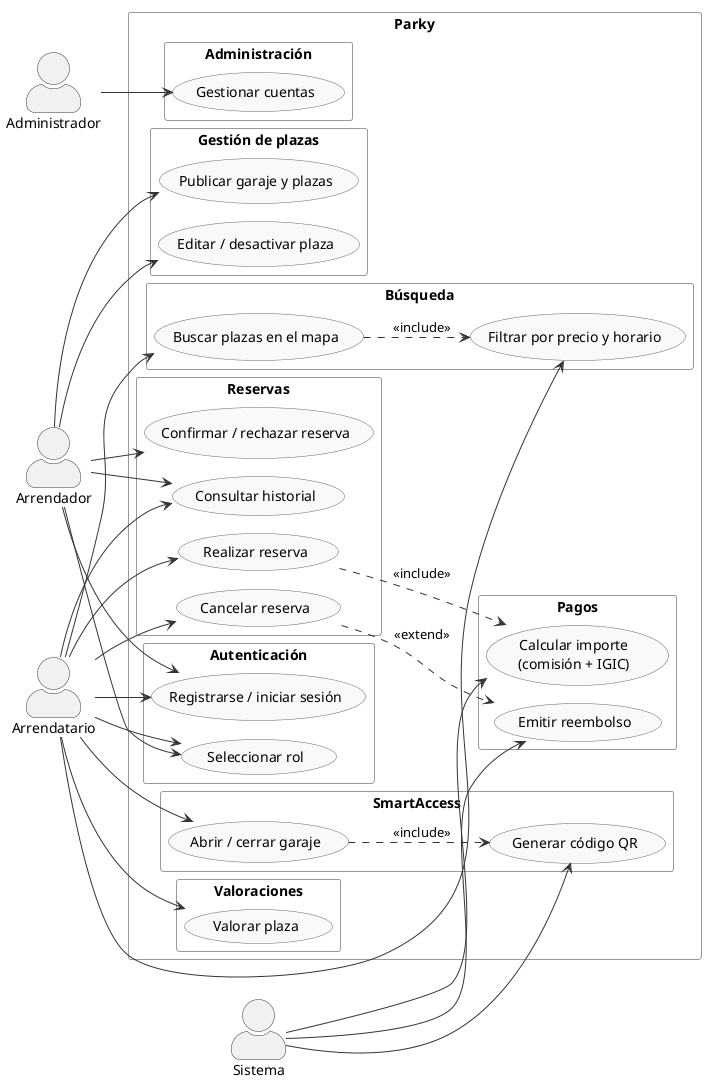
\includegraphics[width=0.48\textwidth]{images/assets/casos_de_uso}
  \caption{Diagrama de casos de uso del sistema Parky.}
  \label{fig:casos_de_uso_uml}
\end{figure}

% ============================================================
\section{Trazabilidad de objetivos}
\label{sec:trazabilidad}
% ============================================================

La Tabla~\ref{tab:trazabilidad} recoge la correspondencia entre los objetivos específicos de la sección~\ref{sec:objetivos}, los requisitos funcionales de la Tabla~\ref{tab:rf} y los casos de uso de la sección~\ref{sec:casos_de_uso}, mostrando que todos los objetivos quedan cubiertos por al menos un requisito y un caso de uso verificable.

\begin{table}[htbp]
  \centering
  \caption{Matriz de trazabilidad: objetivo específico \textrightarrow\ req. funcional \textrightarrow\ caso de uso.}
  \label{tab:trazabilidad}
  \begin{tabularx}{\textwidth}{lXX}
    \toprule
    \textbf{Objetivo}                         & \textbf{Req. funcionales}                                   & \textbf{Casos de uso} \\
    \midrule
    \rowcolor{gray!5}
    OE1 — Autenticación y RBAC                & RF-01, RF-02                                                & CU-01                 \\
    OE2 — SPA, mapa y geocodificación         & RF-03, RF-04, RF-13                                         & CU-02, CU-03          \\
    \rowcolor{gray!5}
    OE3 — Aislamiento RLS                     & RF-03 a RF-15 (operaciones sobre datos propios de cada rol) & CU-01 a CU-04         \\
    OE4 — Integridad de reservas              & RF-05, RF-06                                                & CU-04                 \\
    \rowcolor{gray!5}
    OE5 — \textit{Checkout} e IGIC            & RF-08, RF-09                                                & CU-04                 \\
    OE6 — Estados, SmartAccess y valoraciones & RF-07, RF-10, RF-11, RF-12, RF-14, RF-15                    & CU-04                 \\
    \rowcolor{gray!5}
    OE7 — Despliegue web y Android            & RF-01 a RF-16                                               & CU-01 a CU-04         \\
    \bottomrule
  \end{tabularx}
\end{table}

% ============================================================
\section{Diseño de la base de datos}
\label{sec:diseno-bd}

La base de datos se ejecuta sobre PostgreSQL~15 en Supabase. El esquema normaliza cada entidad de negocio en tablas independientes vinculadas por \textit{foreign keys}. La tabla \texttt{profiles} almacena la información de cada usuario, incluyendo su rol (arrendador o arrendatario) y datos de contacto. La tabla \texttt{garages} representa los garajes publicados por los arrendadores, con su dirección y geolocalización. Cada garaje puede tener varias plazas, por lo que se almacenan en la tabla \texttt{parking\_spots}, que incluye precio por hora y disponibilidad y se relaciona con \texttt{garages} mediante una \textit{foreign key}. Las reservas se registran en la tabla \texttt{bookings} con su estado y ventana temporal, mientras que las valoraciones de los arrendatarios se almacenan en la tabla \texttt{reviews}. El modelo de pagos se apoya en la tabla \texttt{transactions}, que registra el importe, comisión e IGIC de cada reserva confirmada.

% ------------------------------------------------------------
% ------------------------------------------------------------
\subsection{Diagrama de la base de datos}
\label{subsec:diagramas}

\begin{figure}[H]
  \centering
  \hspace*{-6cm}
  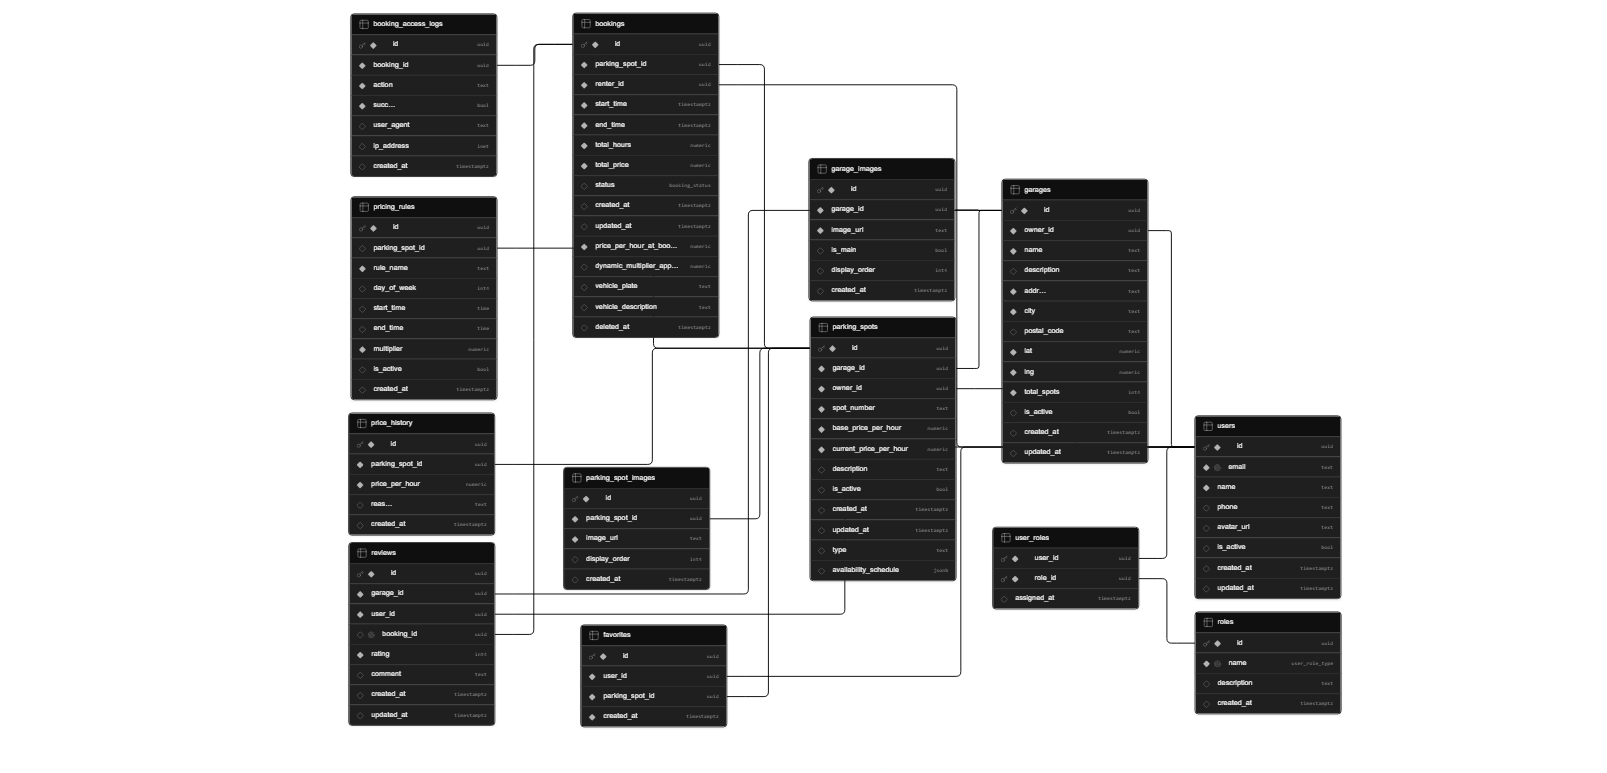
\includegraphics[width=1.15\textheight,keepaspectratio]{images/assets/Diagrama_ER}
  \caption{Diagrama entidad-relación del esquema de base de datos de Parky.}
  \label{fig:er-diagram}
\end{figure}

% ------------------------------------------------------------
\subsection{Políticas RLS}
\label{subsec:rls}

Las políticas de \textit{Row Level Security} (RLS) de PostgreSQL filtran automáticamente las filas que cada usuario puede leer o modificar antes de devolver cualquier resultado, sin que el código del cliente intervenga. Esto significa que aunque un arrendatario manipulara la petición para incluir el identificador de otro usuario, la base de datos rechazaría la operación sin necesidad de ninguna validación adicional en el servidor de aplicación. Las cuatro políticas principales de Parky se recogen en la Tabla~\ref{tab:rls-policies}: cada una vincula el acceso a la identidad autenticada mediante \texttt{auth.uid()}, de modo que arrendadores y arrendatarios operan sobre subconjuntos de datos completamente aislados entre sí.

\begin{table}[htbp]
  \centering
  \caption{Políticas de seguridad a nivel de fila (RLS) del esquema de Parky.}
  \label{tab:rls-policies}
  \begin{tabularx}{\textwidth}{llX}
    \toprule
    \textbf{Tabla}    & \textbf{Operación} & \textbf{Condición de acceso}                                                                                       \\
    \midrule
    \rowcolor{gray!5}
    \texttt{profiles} & SELECT, UPDATE     & Solo el propio usuario puede leer o modificar su perfil (\texttt{auth.uid() = user\_id}).                          \\
    \texttt{bookings} & SELECT             & Arrendador: ve reservas de sus plazas. Arrendatario: solo sus propias reservas (\texttt{tenant\_id = auth.uid()}). \\
    \rowcolor{gray!5}
    \texttt{bookings} & INSERT             & Solo usuarios con rol \texttt{arrendatario} pueden crear reservas a su nombre.                                     \\
    \texttt{reviews}  & INSERT             & Solo si la reserva referenciada pertenece al usuario y está en estado \texttt{completada}.                         \\
    \bottomrule
  \end{tabularx}
\end{table}

% ------------------------------------------------------------
\subsection{Trigger de integridad de reservas}
\label{subsec:triggers}

La tabla \texttt{bookings} está protegida por dos triggers que garantizan la integridad de las reservas a nivel de base de datos. El primero, \texttt{prevent\_booking\_overlap}, impide que se creen dos reservas solapadas en la misma plaza: antes de evaluar el solapamiento, el trigger adquiere un bloqueo explícito sobre la fila de \texttt{parking\_spots} correspondiente mediante \texttt{SELECT \ldots FOR UPDATE}, serializando el acceso concurrente a la misma plaza y garantizando que dos transacciones simultáneas no pasan el chequeo de forma simultánea bajo el nivel de aislamiento \texttt{READ COMMITTED} que PostgreSQL usa por defecto. Adicionalmente, aplica un espaciado de 15 minutos entre reservas consecutivas (con el fin de garantizar el tiempo necesario a sacar el coche o en su defecto a la grúa). El segundo, \texttt{enforce\_booking\_status\_machine}, restringe las transiciones del estado de la reserva a la secuencia \texttt{pendiente} $\to$ \texttt{confirmada} $\to$ \texttt{activa} $\to$ \texttt{completada}, impidiendo que una reserva cancelada pueda reactivarse.


PostgreSQL permite una alternativa para detectar solapamientos temporales mediante restricciones \texttt{EXCLUDE} con rangos de tipo \texttt{tstzrange} e índices GiST. Esta opción fue considerada y descartada por dos razones. La primera es que las restricciones \texttt{EXCLUDE} se limitan a comparar rangos y no admiten lógica adicional dentro de la misma expresión, de modo que incorporar el buffer de 15 minutos habría requerido una función de comparación personalizada, añadiendo complejidad sin beneficio claro. La segunda es que el trigger produce mensajes de error estructurados que la capa de aplicación puede interpretar directamente para mostrar al conductor el motivo del rechazo, mientras que una violación de restricción \texttt{EXCLUDE} devuelve un error genérico de integridad referencial.
